% cd ..\..\Users\NikitaSkybytskyi\Desktop\c3s2\ecology-and-economics\eco-lab-2\tex
% cls && pdflatex report.tex && cls && pdflatex report.tex && del report.aux, report.toc, report.log, report.out && start report.pdf
\documentclass[12pt, a4paper]{article}
\usepackage[T2A]{fontenc}
\usepackage[utf8]{inputenc}
\usepackage[english,ukrainian]{babel}
\usepackage{amsmath, amssymb}

\usepackage[top = 2 cm, left = 1 cm, right = 1 cm, bottom = 2 cm]{geometry}

\usepackage{float, graphicx}

\usepackage{minted}

\newcommand*\diff{\mathop{}\!\mathrm{d}}

\setlength\parindent{0pt}
\allowdisplaybreaks

\newcommand{\cover}[2]{
\begin{center}
\hfill \break
	Міністерство освіти та науки України \\
	Київський національний університет імені Тараса Шевченка \\ 
	Факультет комп'ютерних наук та кібернетики \\
	Кафедра обчислювальної математики
\end{center}

\vfill 

\begin{center}
	\large{
		Звіт до лабораторної роботи №{#1} на тему: \\ 
		``{#2}'
	}
\end{center}

\vfill 

\begin{flushright}
	Виконав студент групи ОМ-3 \\
	Гронь Ілля
\end{flushright}

\vfill 

\begin{center}
    Київ, 2018 
\end{center}

\thispagestyle{empty} 
\newpage
}

\begin{document}

\cover{2}{Модель Лотки---Вольтерра. \\ Внутрішньо-видова конкуренція}

\tableofcontents

\section{Модель Лотки---Вольтерра}

\subsection{Теоретичні відомості}

Пригадаємо, що модель Лотки---Вольтерра описується наступною системою диференціальних рівнянь:
\begin{equation}
	\left\{
		\begin{aligned}
			\dot x &= x \cdot (a - b \cdot y), \\
			\dot y &= y \cdot (d \cdot x - c),
		\end{aligned}
	\right.
\end{equation}
де $a$ --- коефіцієнт розмноження жертв за відсутності хижаків, $c$ --- коефіцієнт природної загибелі хижаків, $b$ --- інтенсивність зменшення жертв при взаємодії двох популяці, $d$ --- інтенсивність нарощування біомаси хижаків при цьому. \medskip

Поклавши $\dot x = \dot y = 0$ знаходимо дві стаціонарні точки: 
\begin{itemize}
	\item тривіальне сідло $(x, y) = (0, 0)$;
	\item нетривіальний центр $(x, y) = \left(\frac{c}{d}, \frac{a}{b}\right)$.
\end{itemize}

Також відомо, що загальний інтеграл системи має вигляд
\begin{equation}
	V = d \cdot x - c \cdot \ln x + b \cdot y - a \cdot \ln y,
\end{equation}
де $V$ --- певна константа, яка визначається початковими умовами.

\subsection{Чисельне моделювання}

Було використано мову програмування \texttt{Python} і модуль \texttt{matplotlib.pyplot}. \medskip

Лістинг коду програми для побудови фазового портрету:
\inputminted{python}{py/phase.py}

Результуючі графіки:

\begin{enumerate}
	\item На квадраті $[0, 1] \times [0, 1]$:
	\begin{figure}
		\centering
		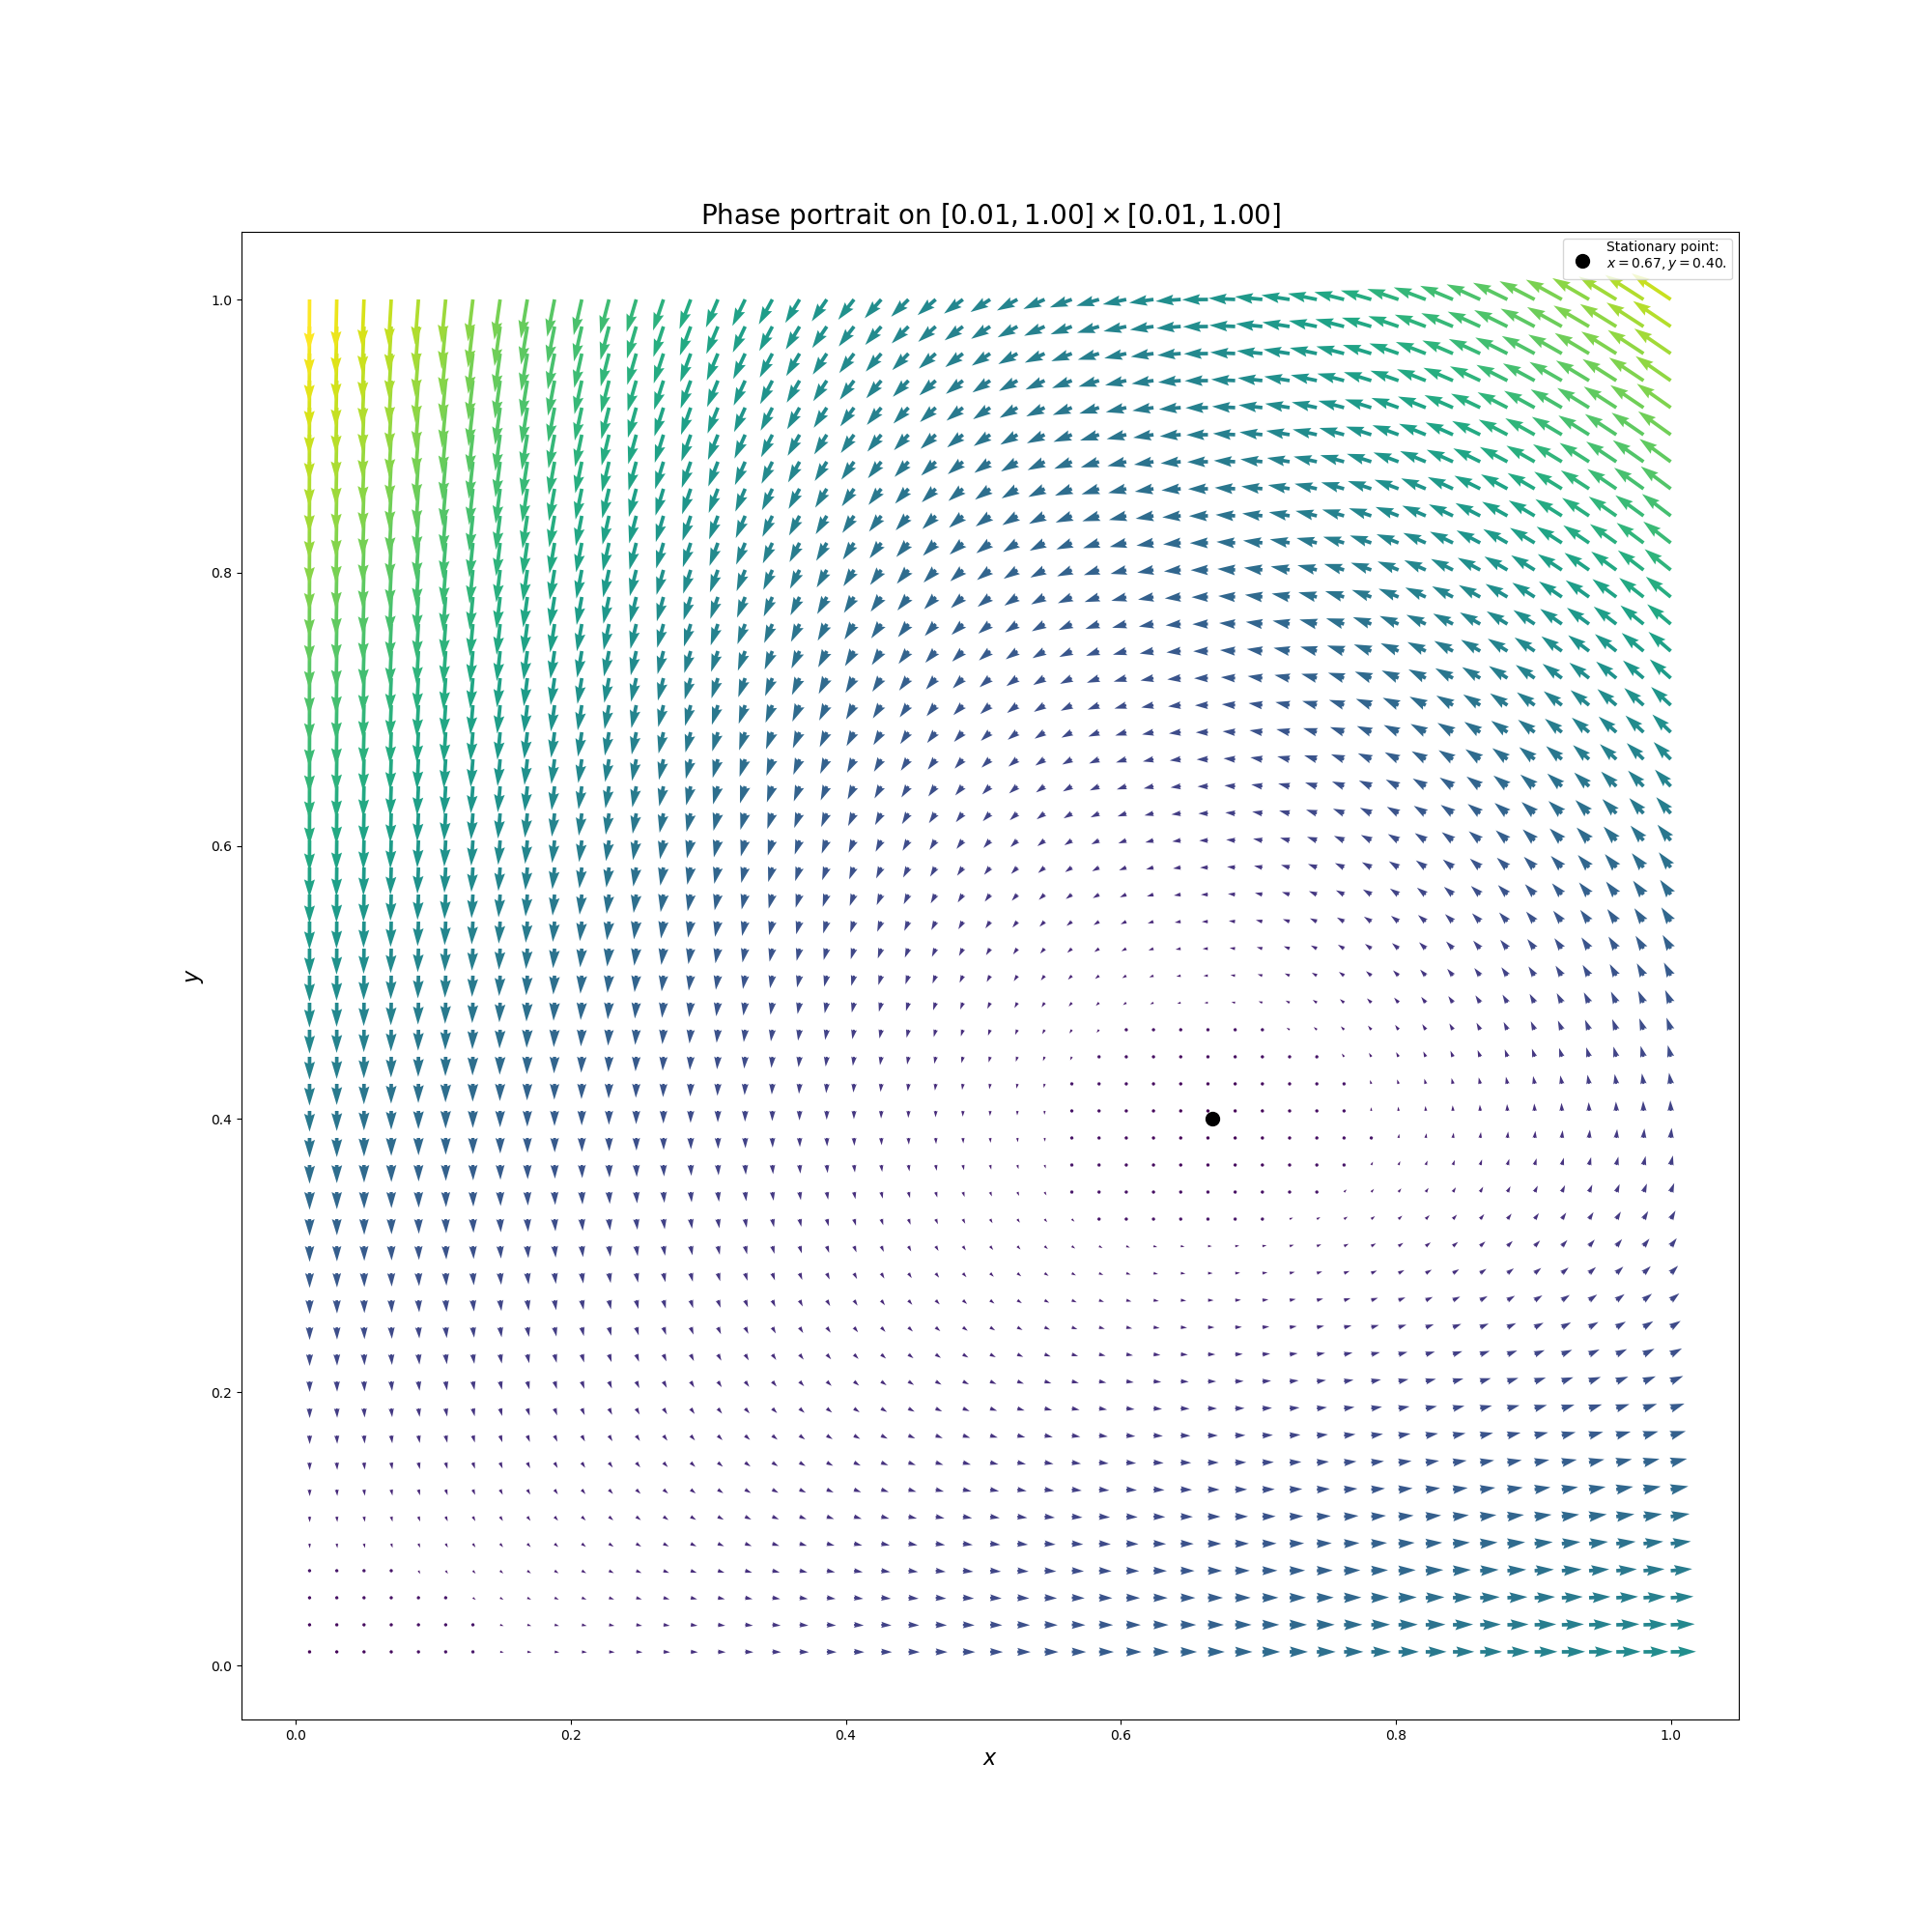
\includegraphics[width=\textwidth]{phase_0.01_1.00_0.01_1.00_50.png}
	\end{figure}

	\item В околі нетривіальної стаціонарної точки:
	\begin{figure}
		\centering
		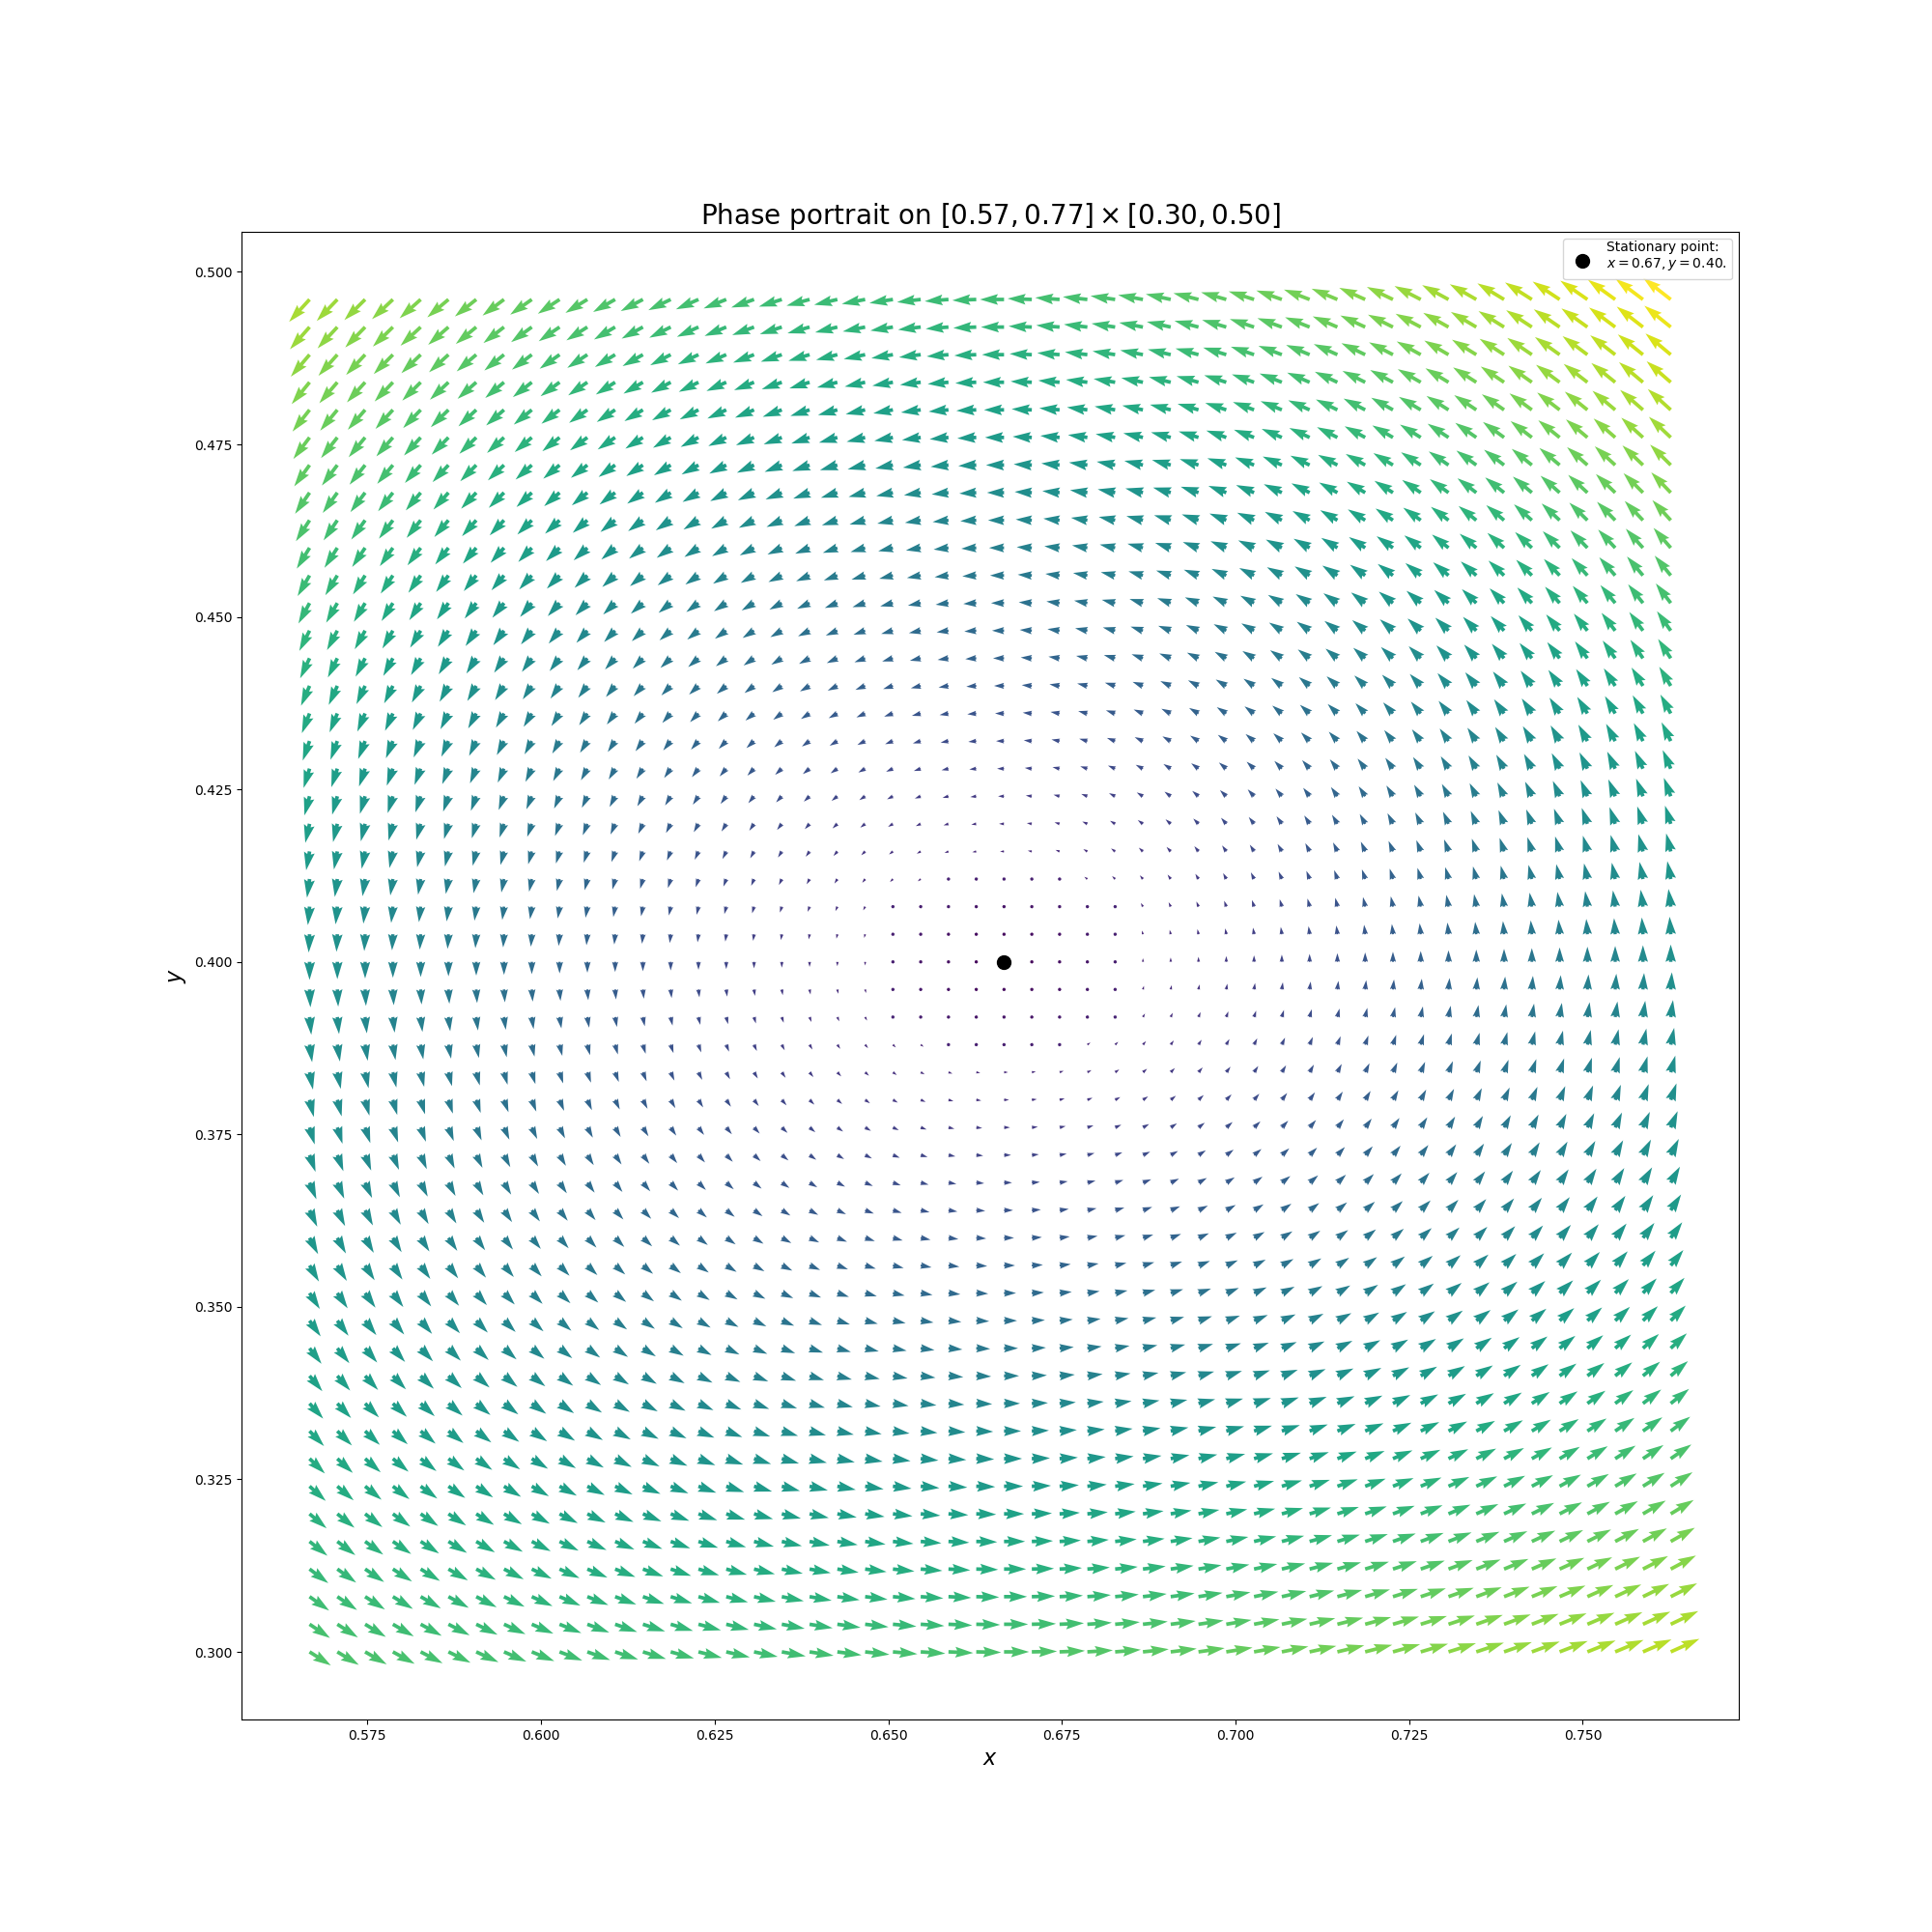
\includegraphics[width=\textwidth]{phase_0.57_0.77_0.30_0.50_50.png}
	\end{figure}

	Зауважимо, що нетривіальна точка --- центр, тому ми також наводимо криві за якими здійснюється обертання.
\end{enumerate}

Як бачимо, отримані результати відповідають теоретичним очікуванням. \medskip

Лістинг коду програми для побудови 2D і 3D графіків чисельності:
\inputminted{python}{py/plots.py}

Результуючі графіки:
\begin{enumerate}
	\item 2D:
	\begin{enumerate}
		\item $x(0) = 0.4$, $y(0) = 0.6$:
		\begin{figure}
			\centering
			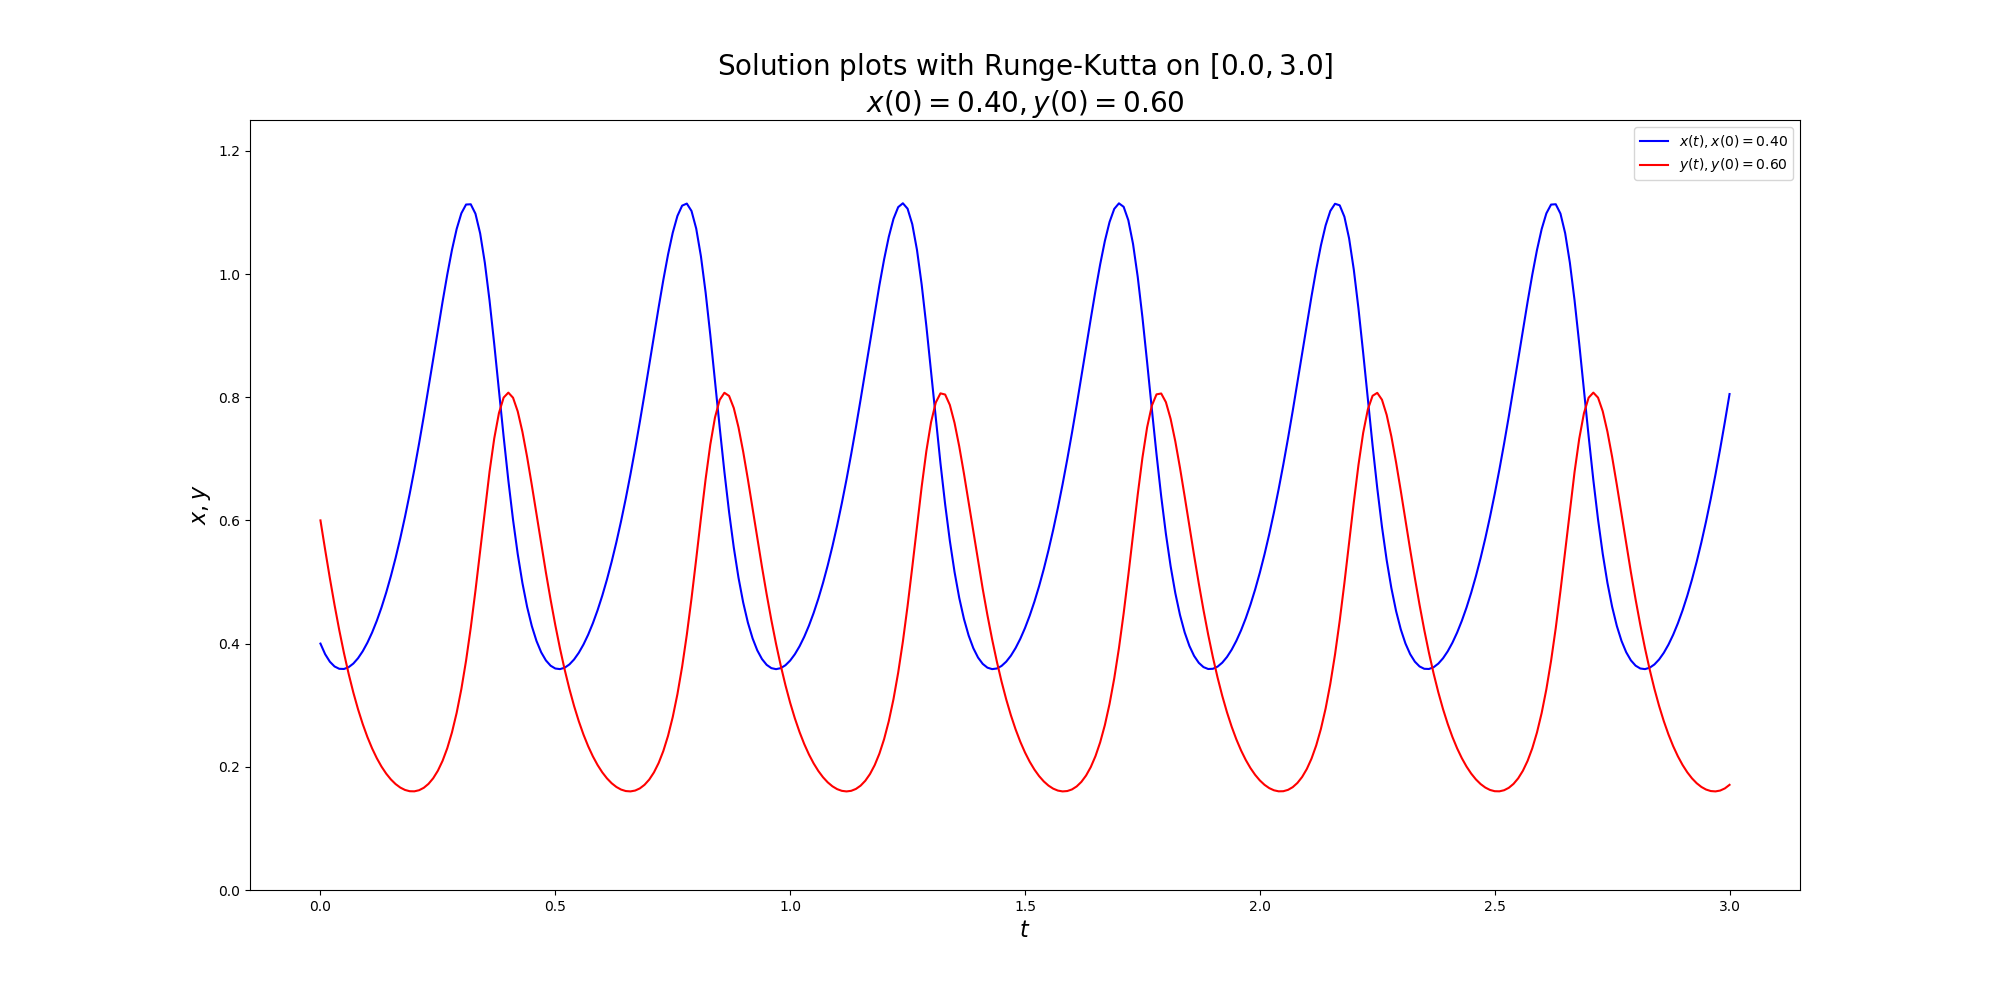
\includegraphics[width=\textwidth]{plot_2d_0.40_0.60.png}
		\end{figure}
		\item $x(0) = 0.5$, $y(0) = 0.5$:
		\begin{figure}
			\centering
			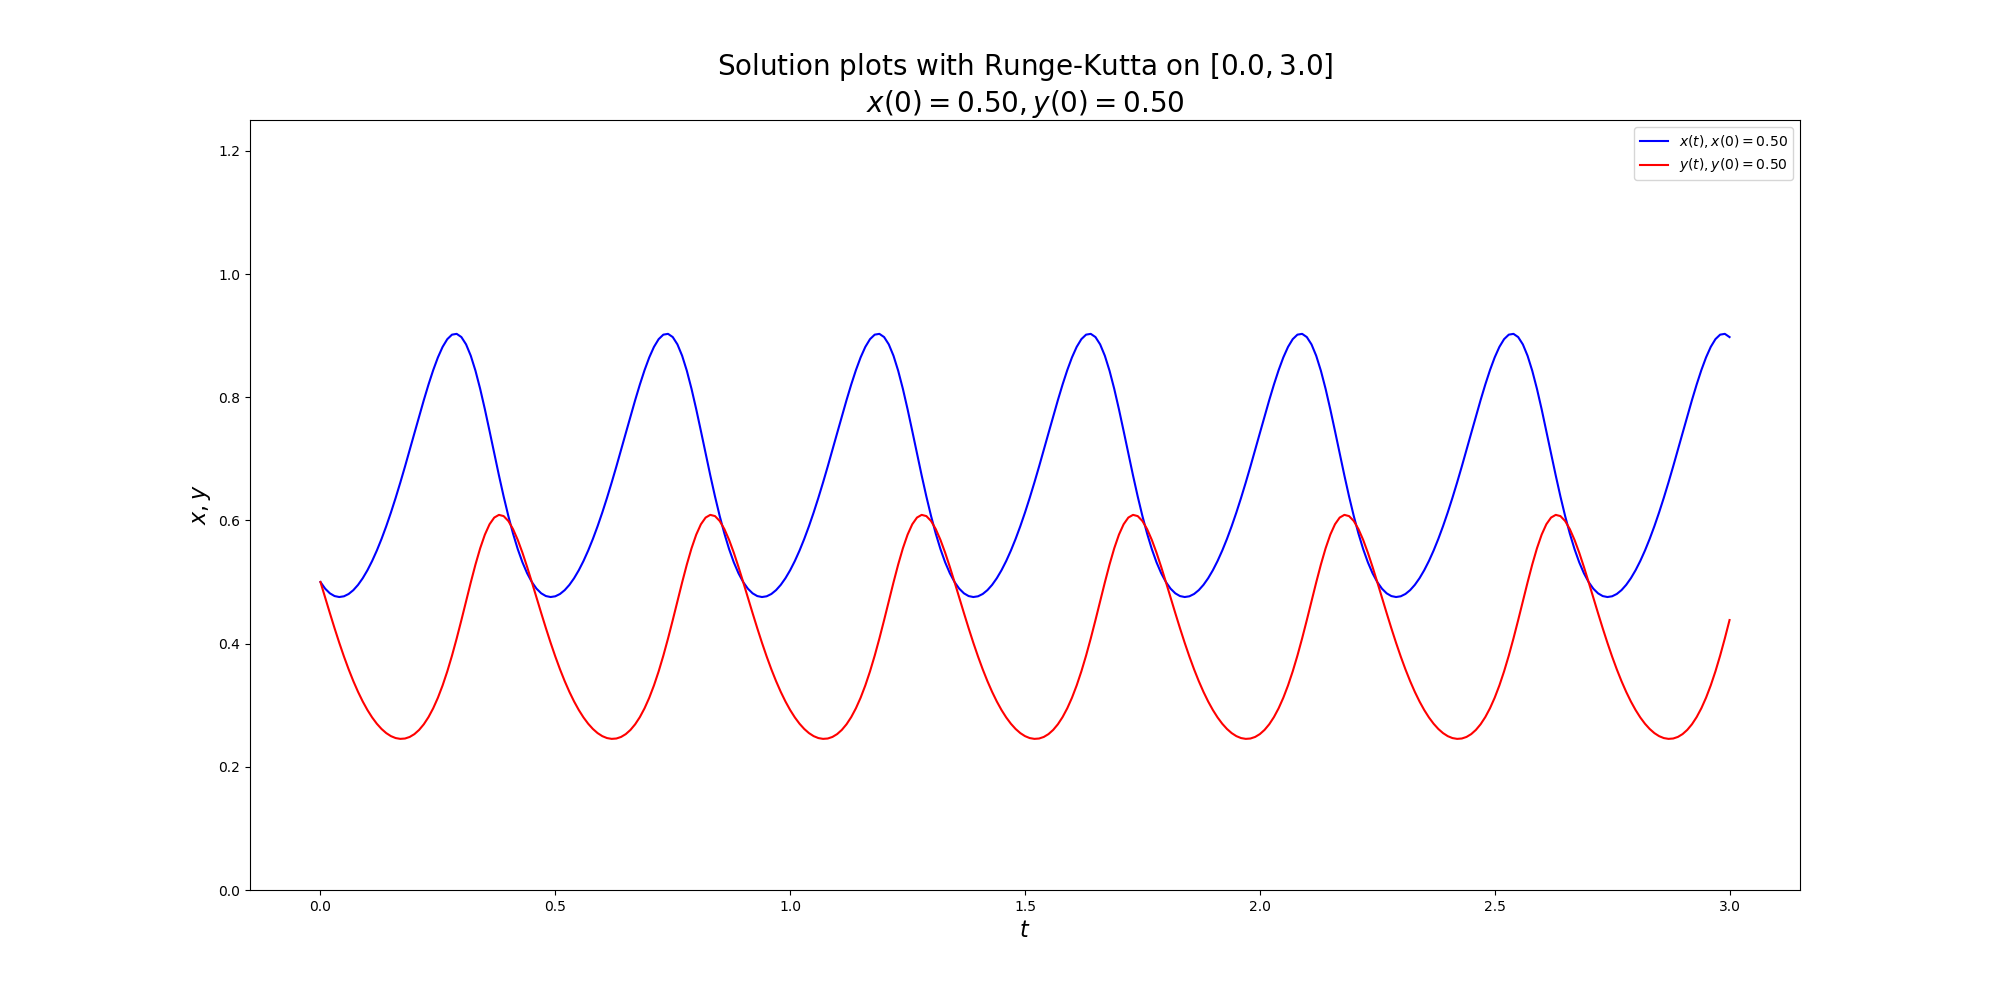
\includegraphics[width=\textwidth]{plot_2d_0.50_0.50.png}
		\end{figure}
		\item $x(0) = 0.8$, $y(0) = 0.2$:
		\begin{figure}
			\centering
			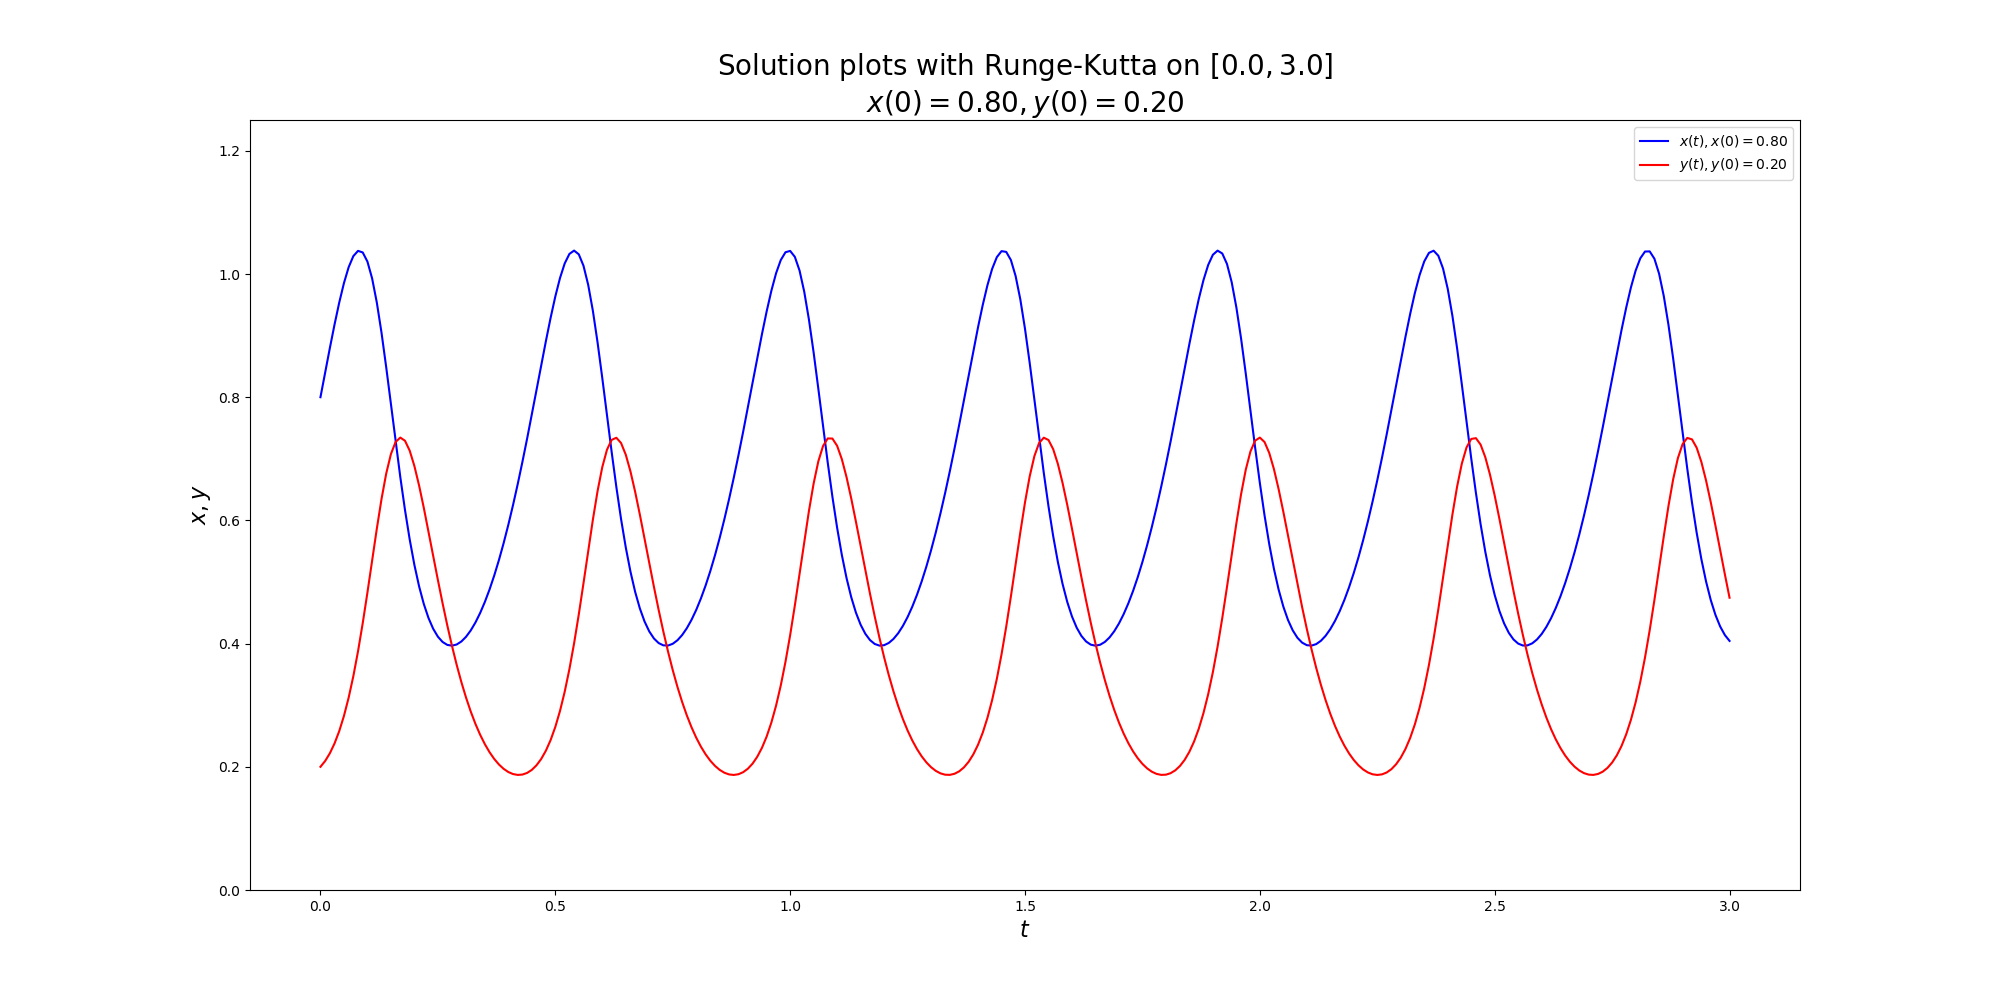
\includegraphics[width=\textwidth]{plot_2d_0.80_0.20.png}
		\end{figure}
	\end{enumerate}
	\item 3D:
	\begin{enumerate}
		\item $x(0) = 0.4$, $y(0) = 0.6$:
		\begin{figure}
			\centering
			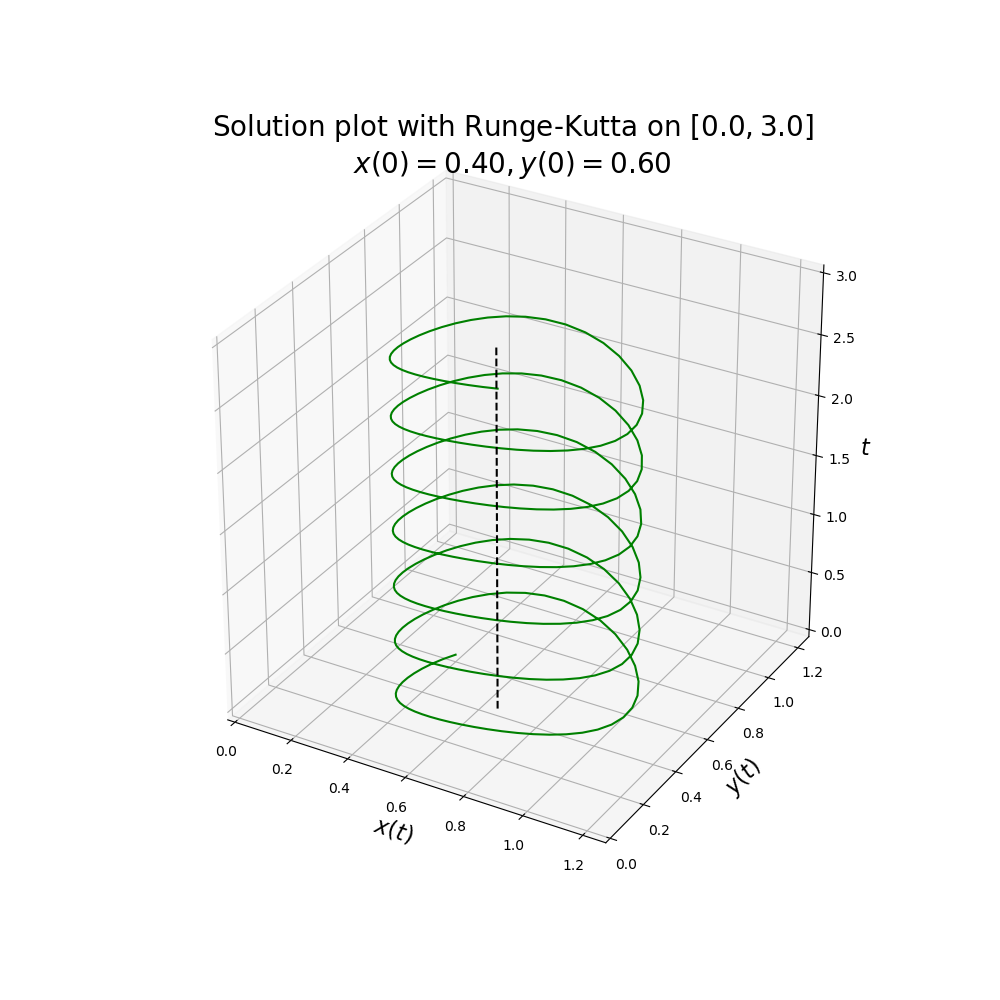
\includegraphics[width=\textwidth]{plot_3d_0.40_0.60.png}
		\end{figure}
		\item $x(0) = 0.5$, $y(0) = 0.5$:
		\begin{figure}
			\centering
			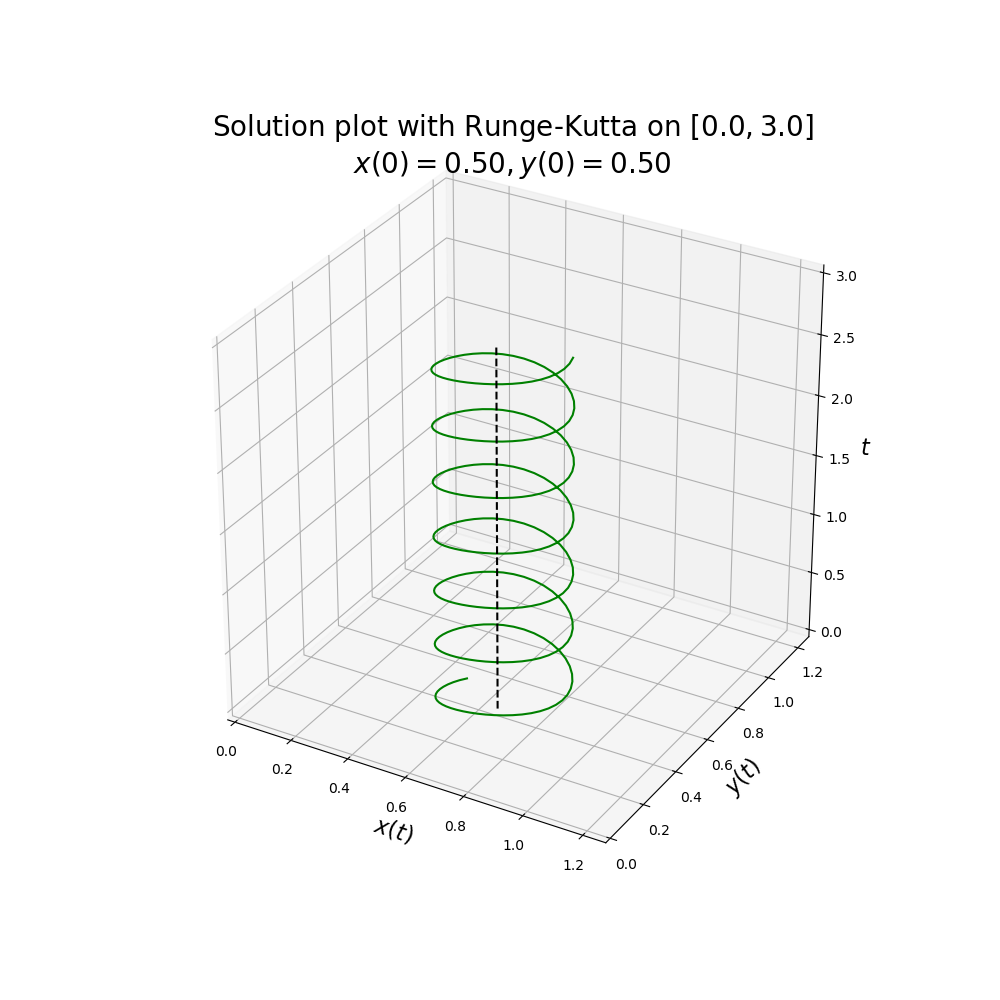
\includegraphics[width=\textwidth]{plot_3d_0.50_0.50.png}
		\end{figure}
		\item $x(0) = 0.8$, $y(0) = 0.2$:
		\begin{figure}
			\centering
			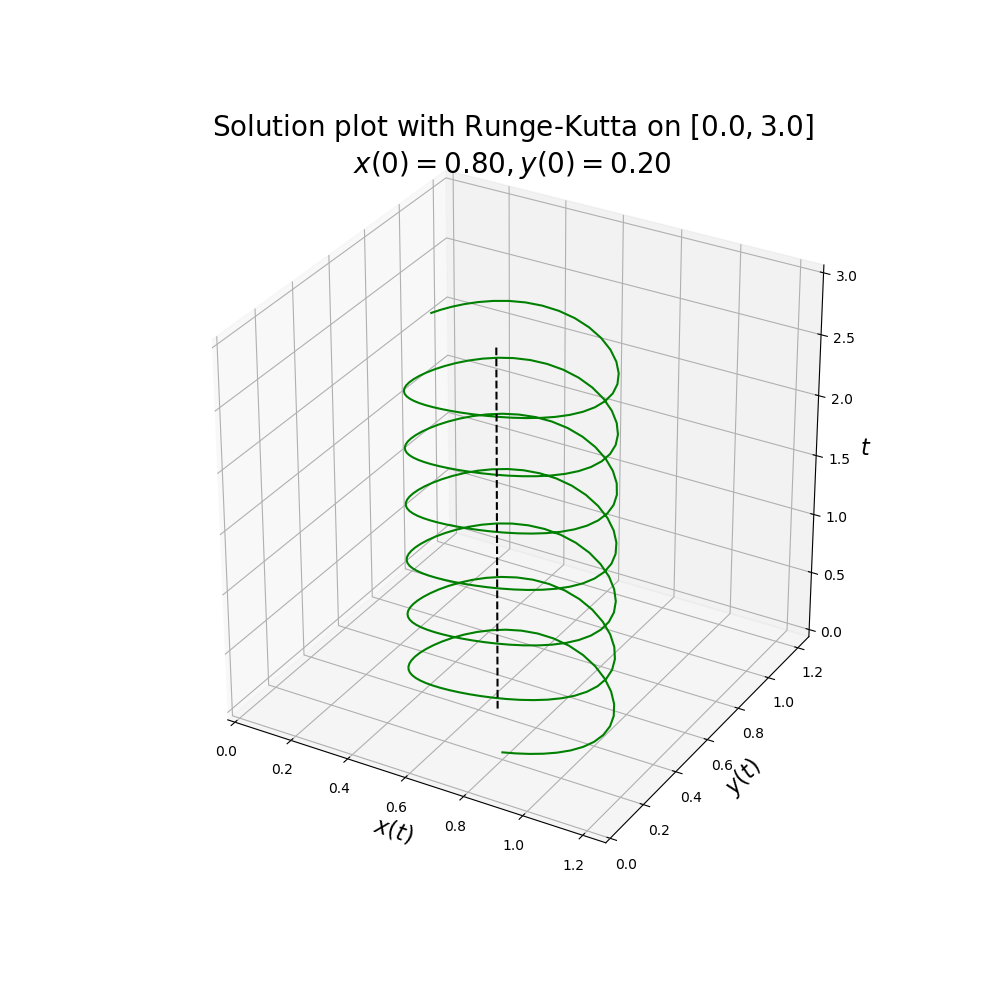
\includegraphics[width=\textwidth]{plot_3d_0.80_0.20.png}
		\end{figure}
	\end{enumerate}
\end{enumerate}

Як бачимо, отримані результати відповідають теоретичним очікуванням. \medskip

\section{Внутрішньо-видова конкуренція}

\subsection{Теоретичні відомості}

Пригадаємо, що модель Лотки---Вольтерра яка враховує внутрішньо-видову конкуренцію описується наступною системою диференціальних рівнянь:
\begin{equation}
	\left\{
		\begin{aligned}
			\dot x &= x \cdot (a - b \cdot y - e \cdot x), \\
			\dot y &= y \cdot (d \cdot x - c),
		\end{aligned}
	\right.
\end{equation}
де $a$ --- коефіцієнт розмноження жертв за відсутності хижаків, $c$ --- коефіцієнт природної загибелі хижаків, $b$ --- інтенсивність зменшення жертв при взаємодії двох популяці, $d$ --- інтенсивність нарощування біомаси хижаків при цьому, і, нарешті, $e$ --- коефіцієнт внутрішньо-видової взаємодії серед жертв. \medskip

Поклавши $\dot x = \dot y = 0$ знаходимо три стаціонарні точки: 
\begin{itemize}
	\item тривіальне сідло $(x, y) = (0, 0)$;
	\item напів-тривіальний стік (eng. \textit{sink}) $(x, y) = \left( \frac{a}{e}, 0 \right)$;
	\item нетривіальний спіральний стік $(x, y) = \left(\frac{c}{d}, \frac{a \cdot d - c \cdot e}{b \cdot d}\right)$.
\end{itemize}

\subsection{Чисельне моделювання}

Було використано мову програмування \texttt{Python} і модуль \texttt{matplotlib.pyplot}. \medskip

Лістинг коду програми для побудови фазового портрету:
\inputminted{python}{py/phase_2.py}

\begin{enumerate}
	\item На квадраті $[0, 1] \times [0, 1]$:
	\begin{figure}
		\centering
		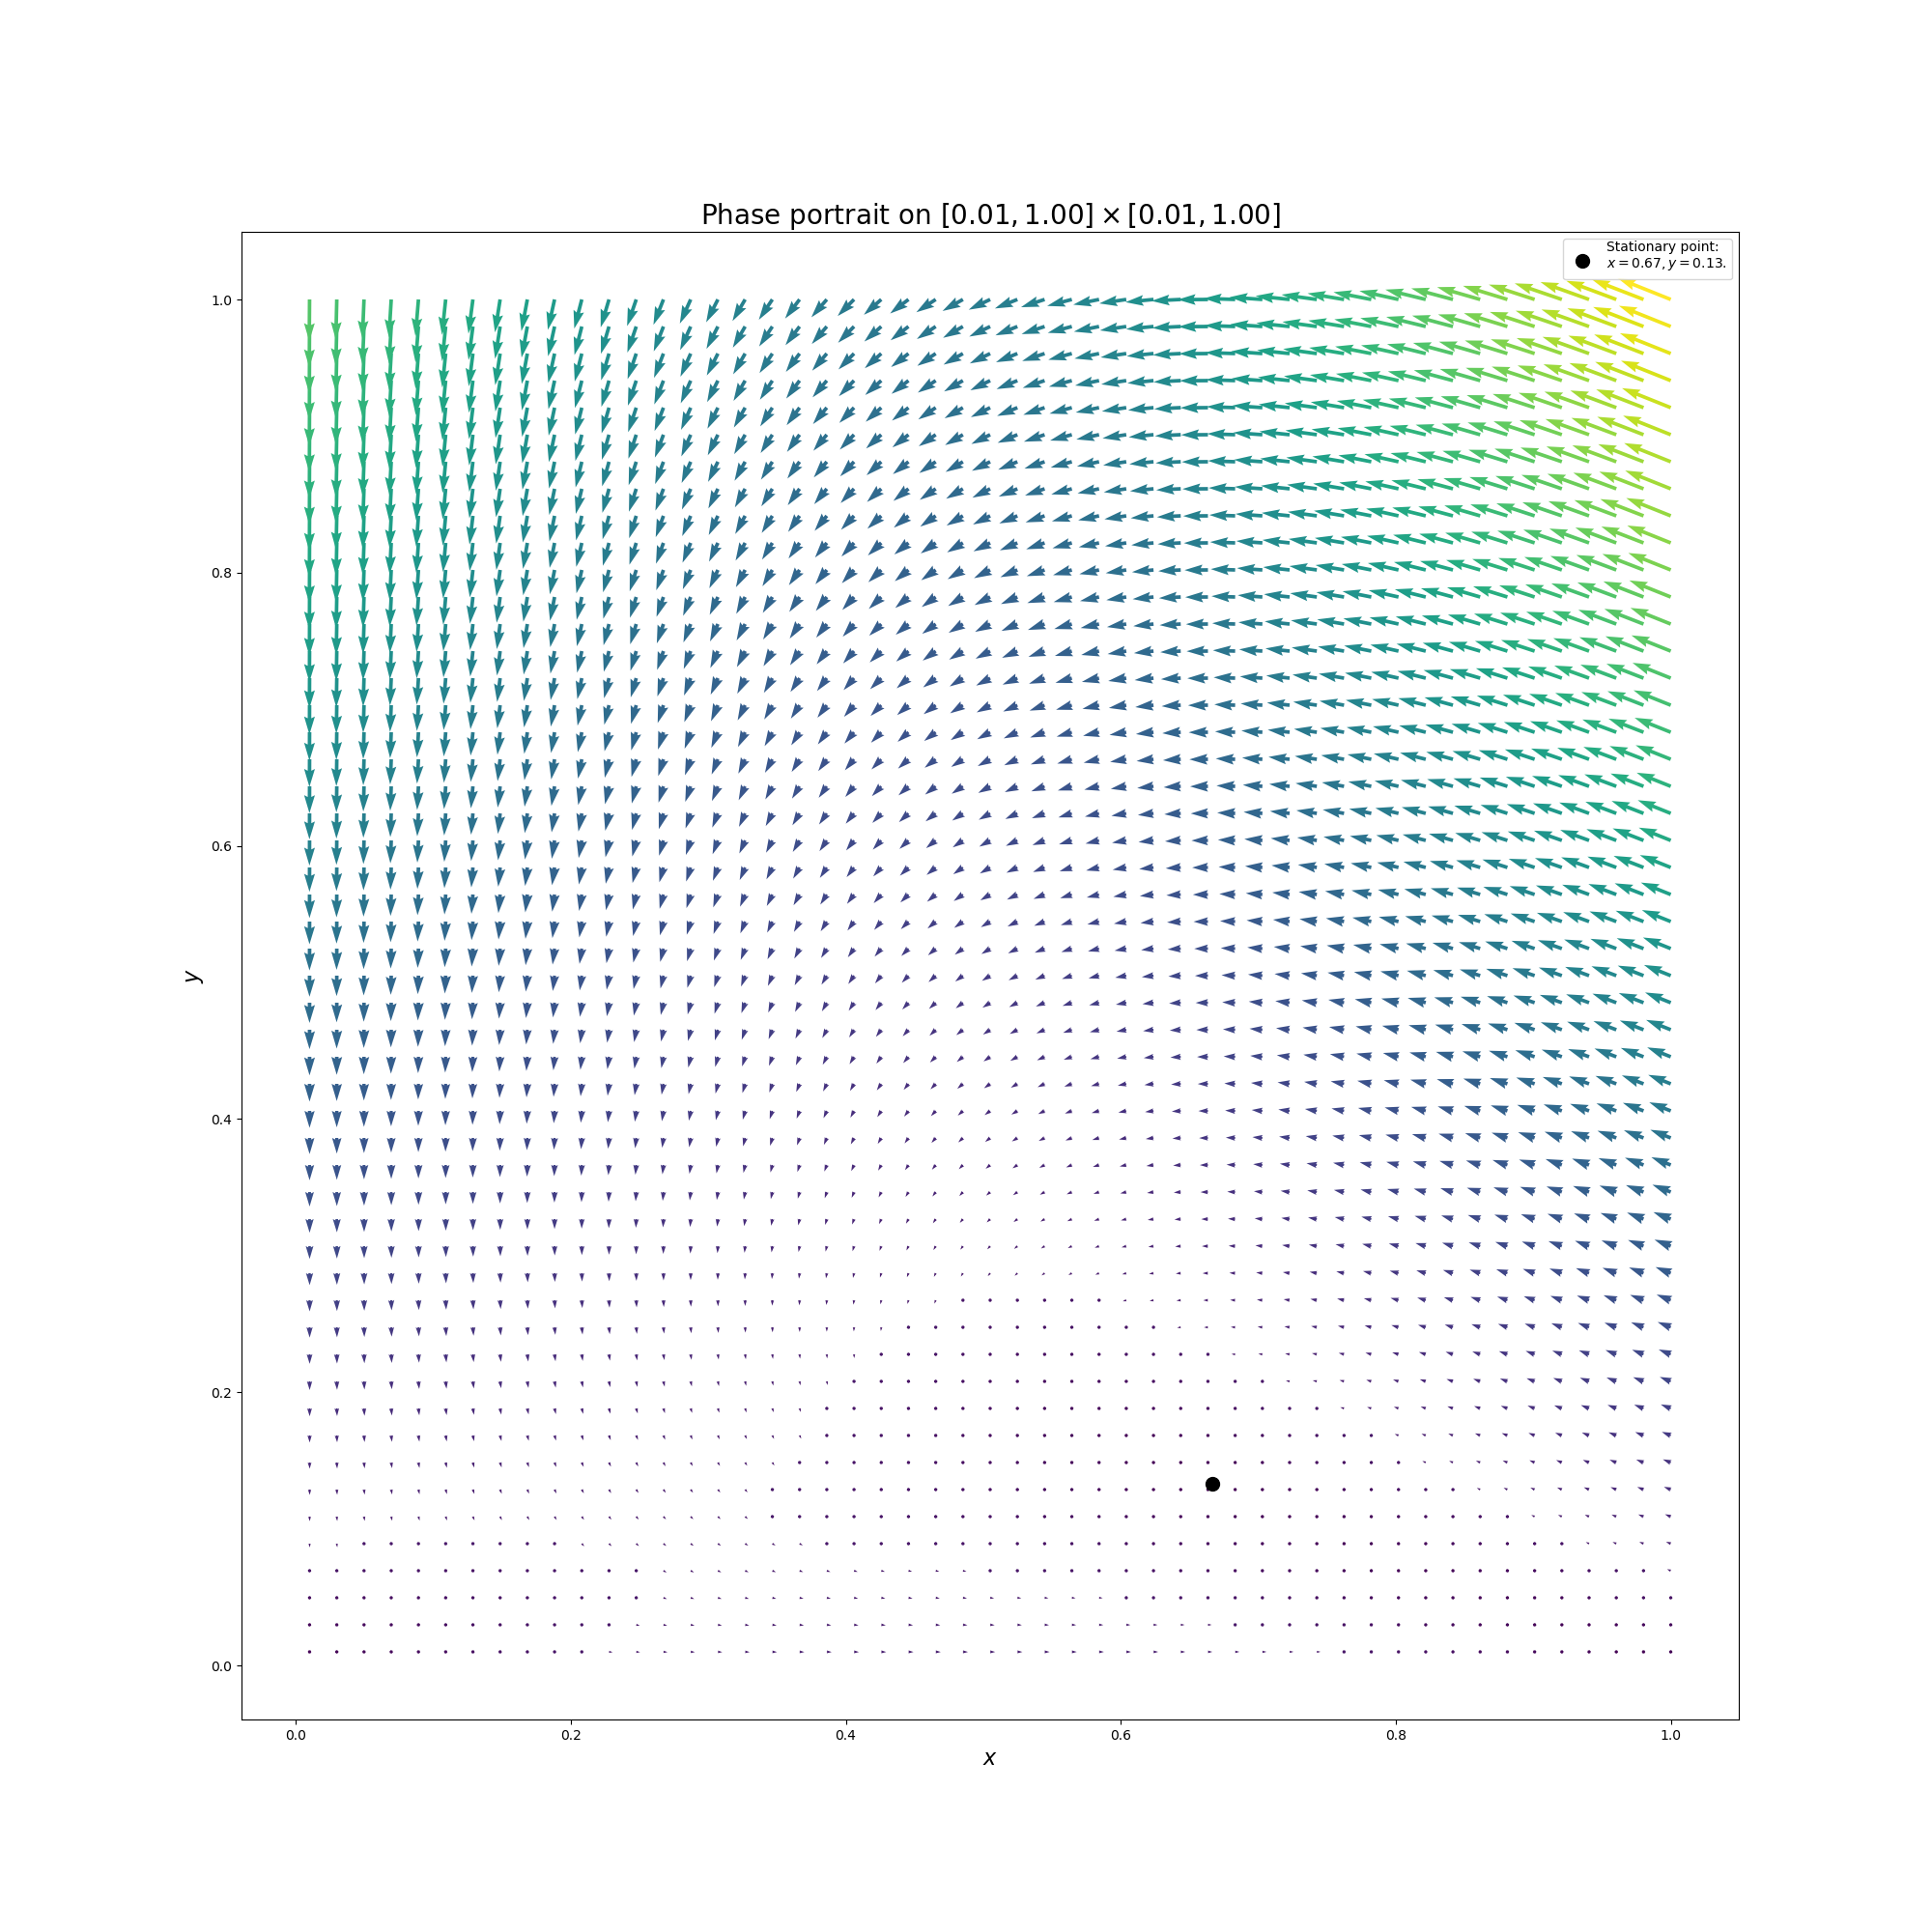
\includegraphics[width=\textwidth]{phase_0.01_1.00_0.01_1.00_50_2.png}
	\end{figure}

	\item В околі нетривіальної стаціонарної точки:
	\begin{figure}
		\centering
		\includegraphics[width=\textwidth]{phase_0.57_0.77_0.03_0.23_50.png}
	\end{figure}
\end{enumerate}

Як бачимо, отримані результати відповідають теоретичним очікуванням. \medskip

Лістинг коду програми для побудови 2D і 3D графіків чисельності:
\inputminted{python}{py/plots_2.py}

Результуючі графіки:
\begin{enumerate}
	\item 2D:
	\begin{enumerate}
		\item $x(0) = 0.1$, $y(0) = 0.9$:
		\begin{figure}
			\centering
			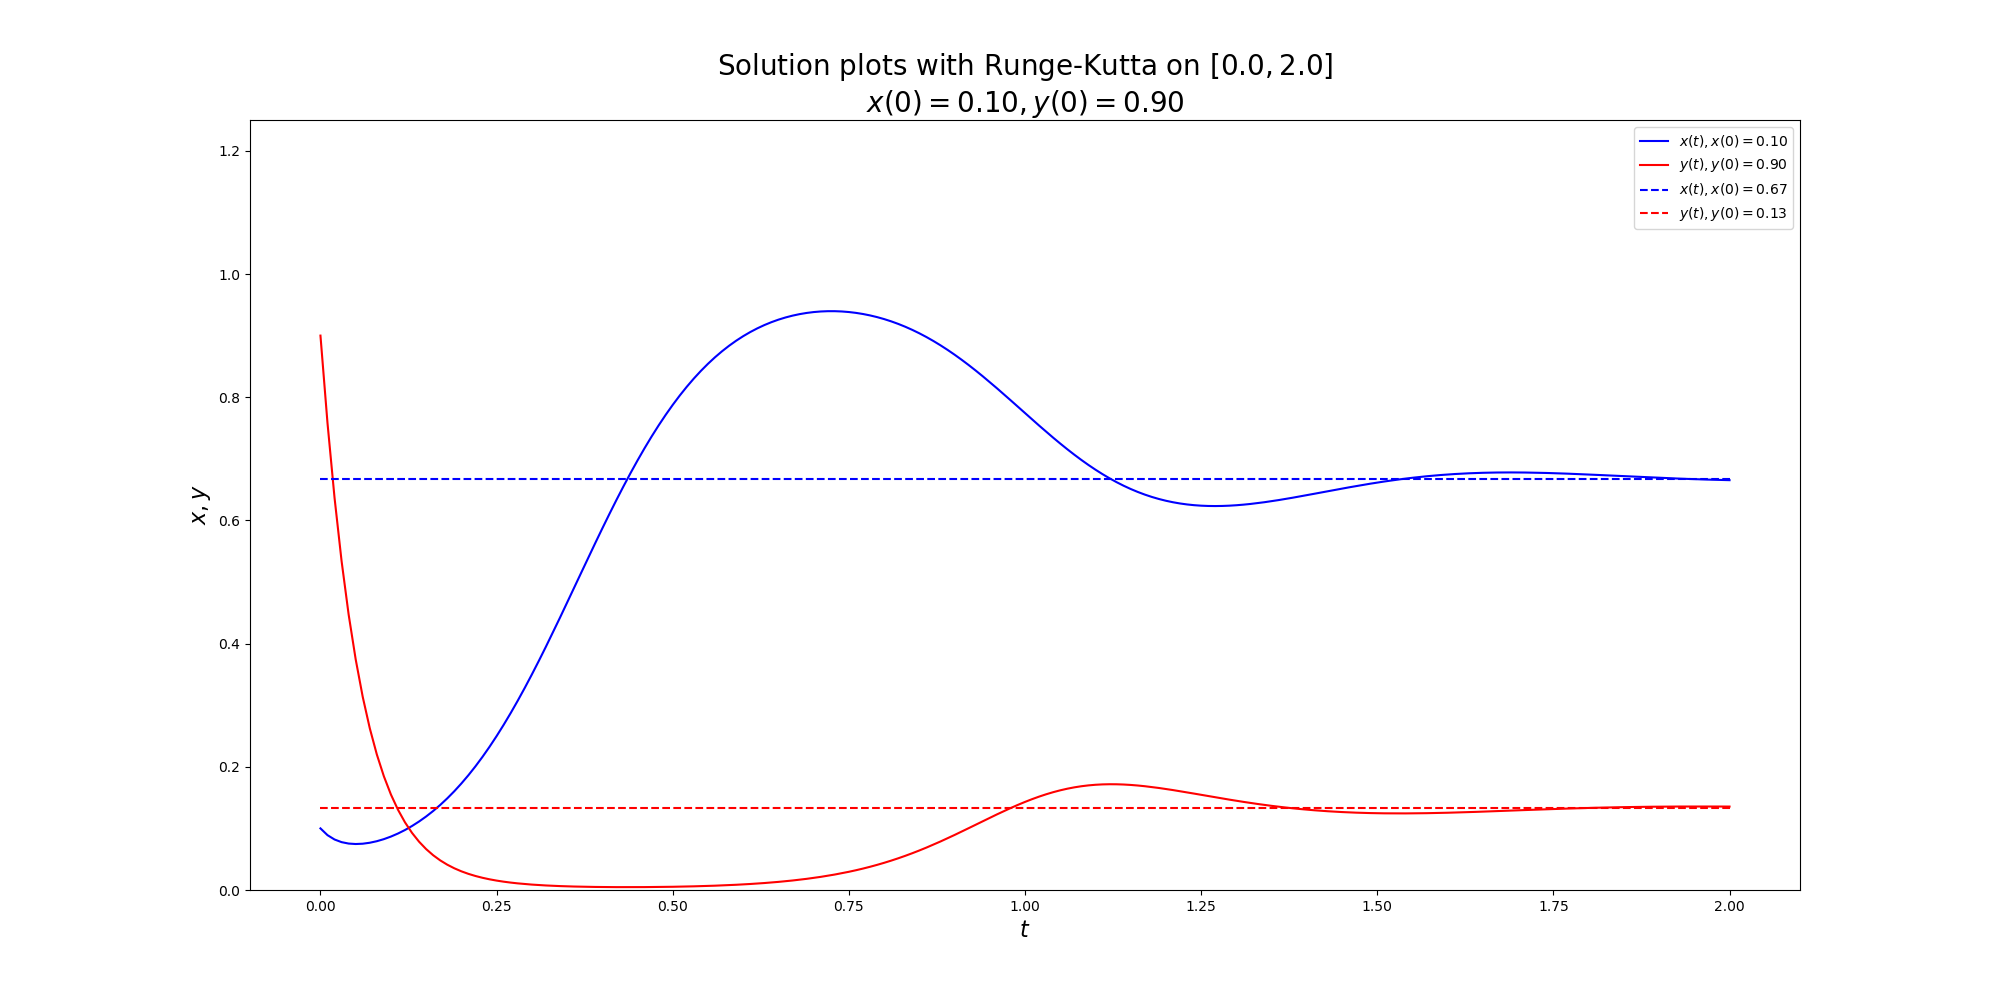
\includegraphics[width=\textwidth]{plot_2d_0.10_0.90_2.png}
		\end{figure}
		\item $x(0) = 0.5$, $y(0) = 0.5$:
		\begin{figure}
			\centering
			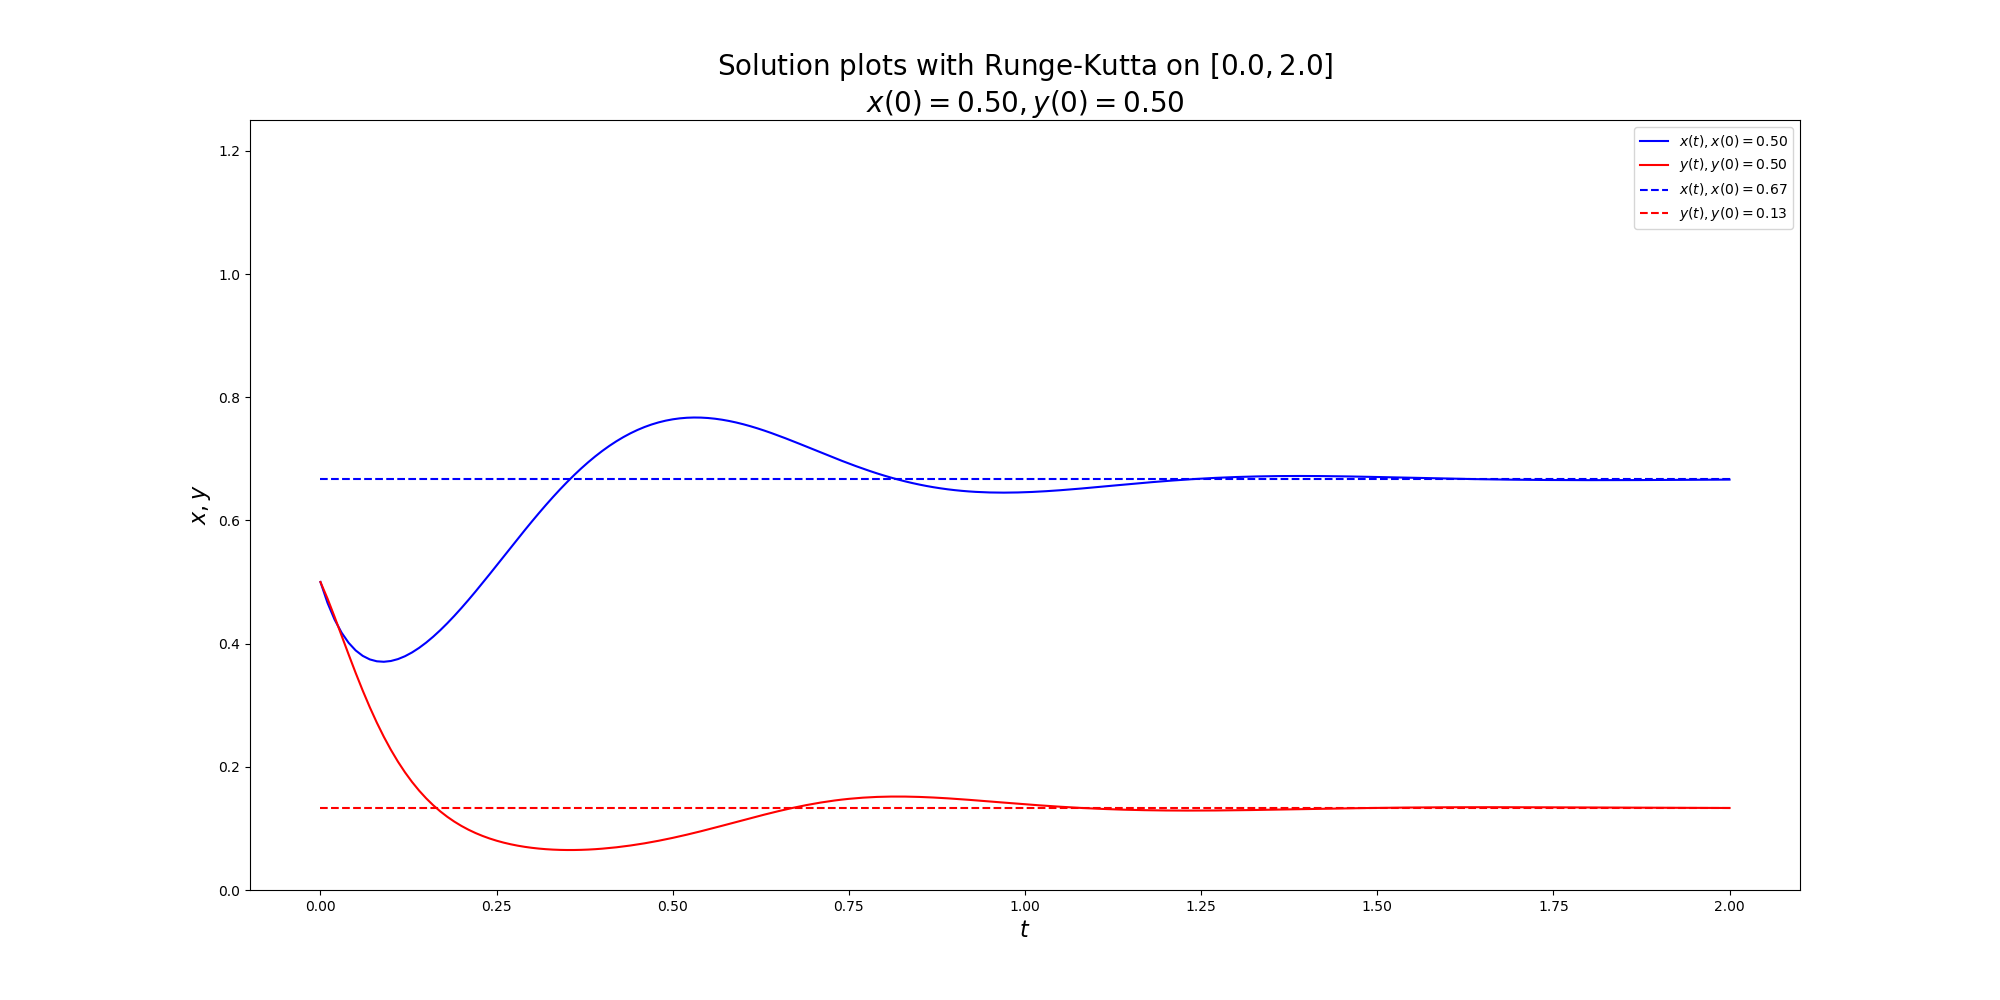
\includegraphics[width=\textwidth]{plot_2d_0.50_0.50_2.png}
		\end{figure}
		\item $x(0) = 0.9$, $y(0) = 0.1$:
		\begin{figure}
			\centering
			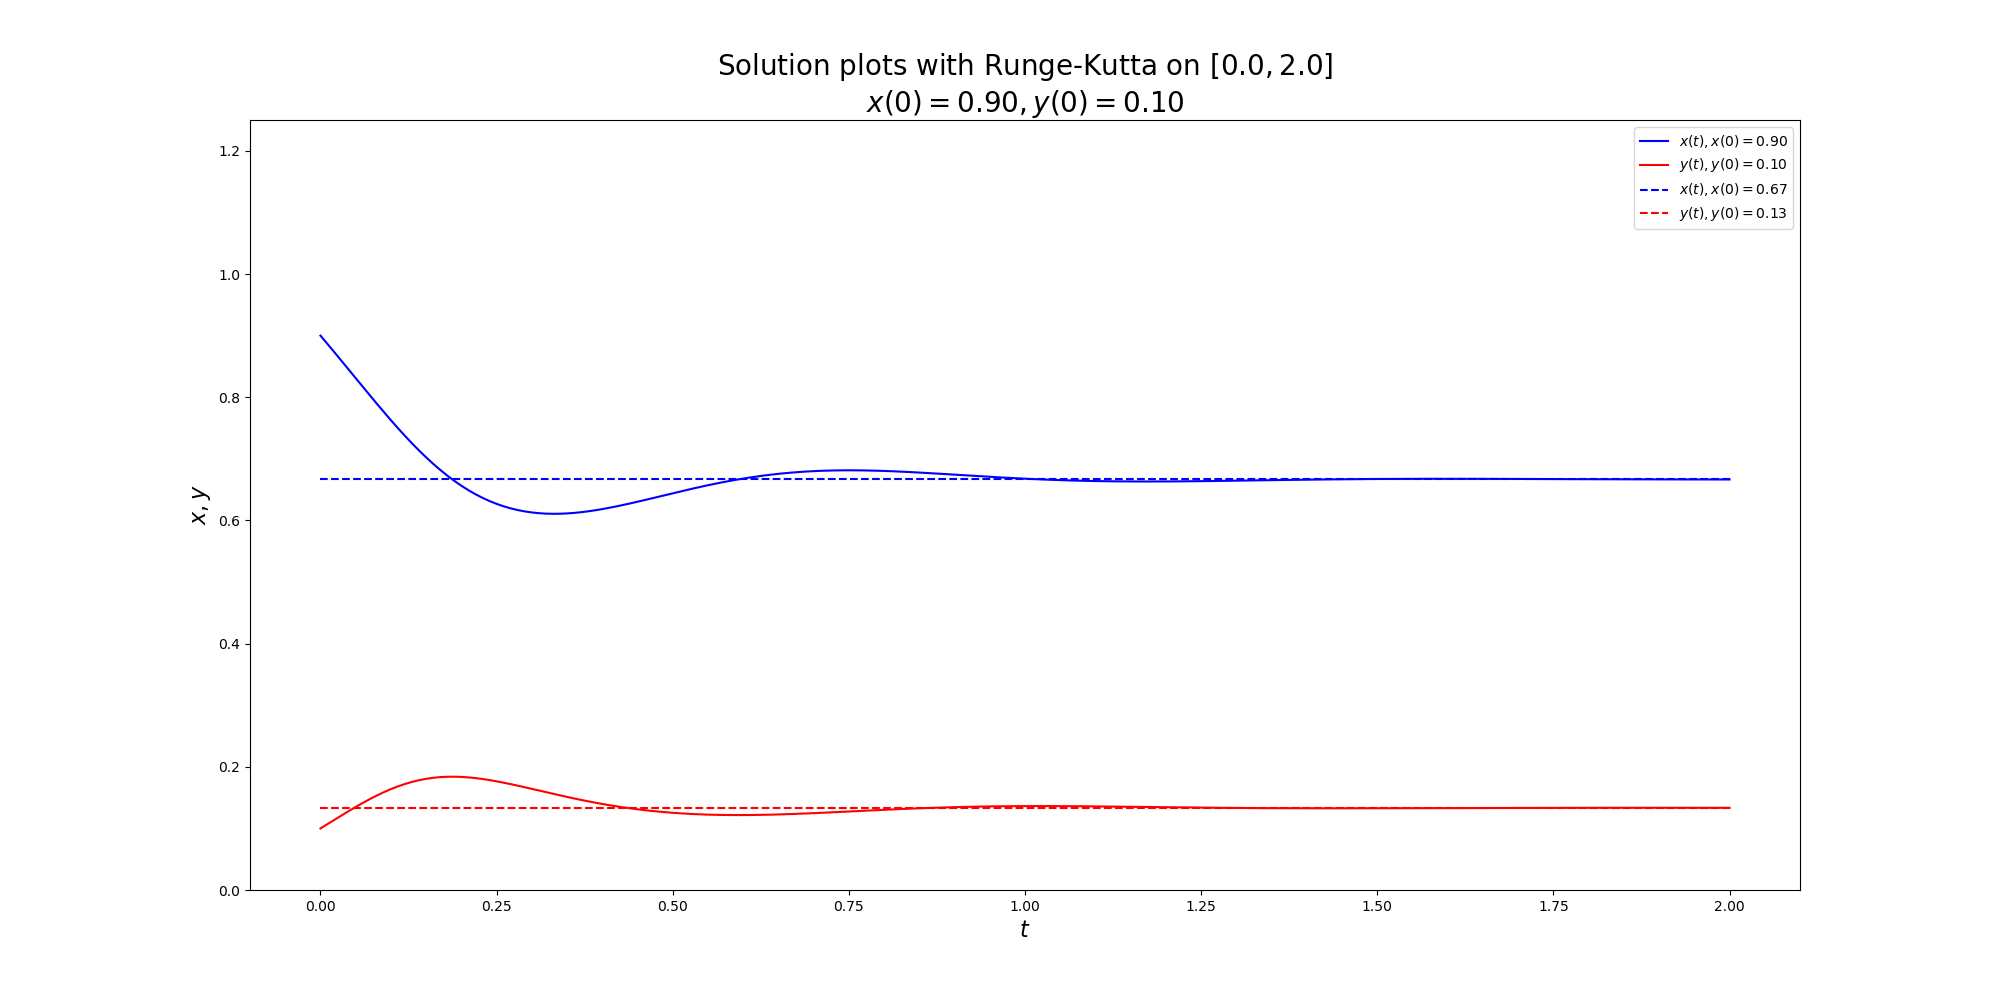
\includegraphics[width=\textwidth]{plot_2d_0.90_0.10_2.png}
		\end{figure}
	\end{enumerate}
	\item 3D:
	\begin{enumerate}
		\item $x(0) = 0.1$, $y(0) = 0.9$:
		\begin{figure}
			\centering
			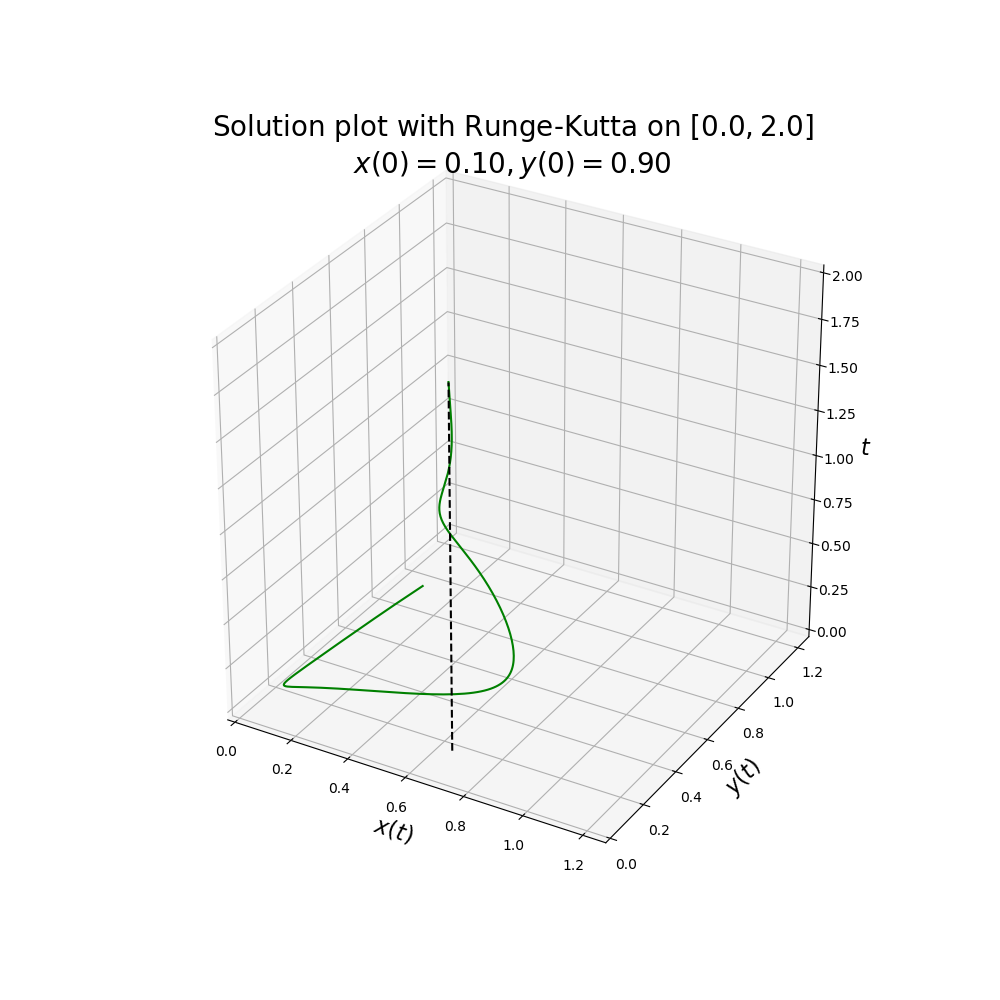
\includegraphics[width=\textwidth]{plot_3d_0.10_0.90_2.png}
		\end{figure}
		\item $x(0) = 0.5$, $y(0) = 0.5$:
		\begin{figure}
			\centering
			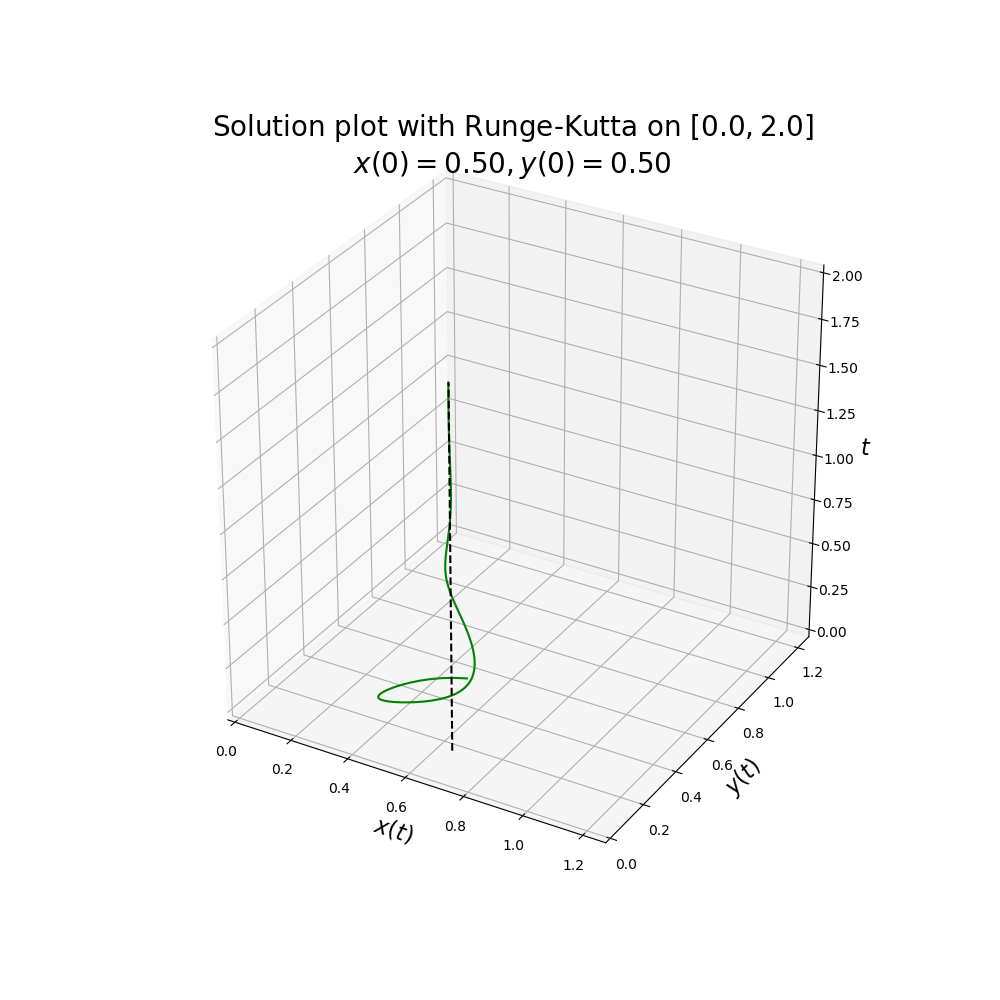
\includegraphics[width=\textwidth]{plot_3d_0.50_0.50_2.png}
		\end{figure}
		\item $x(0) = 0.9$, $y(0) = 0.1$:
		\begin{figure}
			\centering
			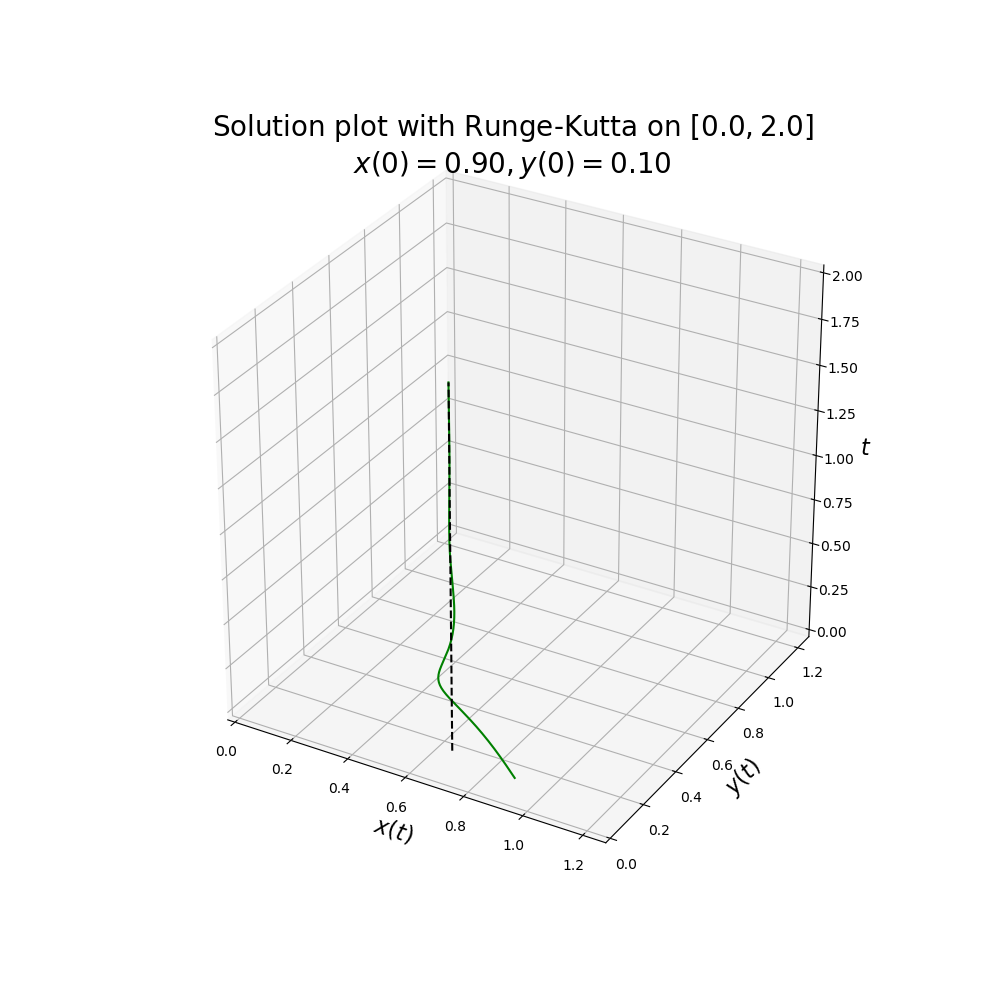
\includegraphics[width=\textwidth]{plot_3d_0.90_0.10_2.png}
		\end{figure}
	\end{enumerate}
\end{enumerate}

Як бачимо, отримані результати відповідають теоретичним очікуванням. \medskip

\end{document}